
\lecture{Central Tendencies}{central-tendencies}
\section{Central Tendencies}

\title{Central Tendencies}
\subtitle{Center and Spread of Data}

%\author{Kelly Black}
%\institute{Clarkson University}
\date{12 February 2014}

\begin{frame}
  \titlepage
\end{frame}

\begin{frame}
  \frametitle{Outline}
  \tableofcontents[hideothersubsections,sectionstyle=show/hide]
\end{frame}


\iftoggle{clicker}{%
  \subsection{Clicker Question}
  \begin{frame}
    \frametitle{Find The Average}
    (Use channel 42)

    \vfill 
    
    \begin{tabular}{lll}
      3, & 5, & -2
    \end{tabular}

    \vfill

    \begin{tabular}{l@{\hspace{3em}}l@{\hspace{3em}}l}
      a: -2 & b: 2 & c: 4
    \end{tabular}

    \vfill


  \end{frame}
}


\subsection{Center of Data}

\begin{frame}{Center of Data}

  {\color{red}The term ``average'' is not a defined quantity.}

  It can mean many things and is misleading!

  Example: \\
  \begin{tabular}{lllllll}
    3, & 5, & -2, & 1 & 10 & -2 & -2
  \end{tabular}

  \uncover<1->%
  {

    It could be the ``sample mean:'' 1.86.

    It could be the ``sample median:'' 1.

    It could be the ``sample mode:'' -2

  }

  
\end{frame}


\begin{frame}{Center of Data}

  What is the ``center'' of the data?

  \begin{tabular}{lll}
    3, & 5, & -2
  \end{tabular}

  
\end{frame}


\begin{frame}{Center of Data}

  What is the ``center?''

  \only<1>{%
    \begin{description}
    \item[Population Mean] The mean of the whole population.
    \item[Sample Mean] The sum of the data divided by the number of
      samples.
    \item[Median] The middle value of the whole population.
    \item[Sample Median] The middle value of the data.
    \end{description}
  }


  \only<2>{%
    \begin{description}
    \item[{\color{red}Population Mean}] {\color{red}The mean of the whole population.*}
    \item[{\color{blue}Sample Mean}] {\color{blue}The sum of the data divided by the number of
      samples.**}
    \item[{\color{red}Median}] {\color{red}The middle value of the whole population.*}
    \item[{\color{blue}Sample Median}] {\color{blue}The middle value of the data.**}
    \end{description}

    {\color{red}What we want.*}

    {\color{blue}What we have.**}

  }

  
\end{frame}



\begin{frame}
  \frametitle{Center of Data}

  Given data:
  \begin{eqnarray*}
    x_1, ~ x_2, ~ x_3, ~ \ldots ~,x_n.
  \end{eqnarray*}

  \begin{definition}[Sample Mean]
    The sample mean of the data is 
    \begin{eqnarray*}
      \bar{x} & = & \frac{x_1+x_2+\cdots+x_n}{n}.
    \end{eqnarray*}
  \end{definition}

  \begin{definition}[Sample Median]
    The sample median is the number for which half the data is smaller
    than it and half is larger than it.
  \end{definition}
  

\end{frame}


\begin{frame}{Example}

  \begin{tabular}{lllllll}
    30 & 28 & 31 & 33 & 35 & 22 & 31
  \end{tabular}

  The sample mean:
  \begin{eqnarray*}
    \bar{x} & = & \frac{30 + 28 + 31 + 33 + 35 + 22 + 31}{7}, \\
    & = & 30.
  \end{eqnarray*}

  To get the sample median first order the data: \\
  \only<1>%
  {
    \begin{tabular}{lllllll}
      22 & 28 & 30 & 31 & 31 & 33 & 35
    \end{tabular}
  }

  \only<2>%
  {
    \begin{tabular}{lllllll}
      {\color{red}22} & {\color{red}28} & {\color{red}30} & 31 & {\color{blue}31} & {\color{blue}33} & {\color{blue}35}
    \end{tabular}
  }

  \only<3->%
  {
    \begin{tabular}{lllllll}
      {\color{red}22} & {\color{red}28} & {\color{red}30} &
      $\underbrace{31}_{Sample~Median}$ & {\color{blue}31} & {\color{blue}33} & {\color{blue}35}
    \end{tabular}
  }
  
\end{frame}


\begin{frame}{Example}

  Even number of data points.

  \begin{tabular}{cccccc}
    30 & 28 & 31 & 33 & 35 & 22 
  \end{tabular}

  The sample mean:
  \begin{eqnarray*}
    \bar{x} & = & \frac{30 + 28 + 31 + 33 + 35 + 22}{6}, \\
    & = & 29.8.
  \end{eqnarray*}

  To get the sample median first order the data: \\
  \only<1>%
  {
    \begin{tabular}{cccccc}
      22 & 28 & 30 & 31 & 33 & 35
    \end{tabular}
  }

  \only<2>%
  {
    \begin{tabular}{cccccc}
      {\color{red}22} & {\color{red}28} & 30 & 31  & {\color{blue}33} & {\color{blue}35}
    \end{tabular}
  }

  \only<3->%
  {
    \begin{tabular}{cccccc}
      {\color{red}22} & {\color{red}28} & 30 & 31 & 
      {\color{blue}33} & {\color{blue}35} \\
      & & \multicolumn{2}{c}{Sample Median = $\frac{30+31}{2}$} 
    \end{tabular}
  }
  
\end{frame}


\begin{frame}
  \frametitle{Clicker Quiz}
  (Use channel 42)

  Find the sample median of the following data set:
  \vfill 

  \begin{tabular}{llll}
    3, & 5, & 2, & 4
  \end{tabular}

  \vfill

  \begin{tabular}{l@{\hspace{3em}}l@{\hspace{3em}}l@{\hspace{3em}}l}
    a: 5/2  & b: 7/2 & c: 3 & D: 4
  \end{tabular}

  \vfill

  

\end{frame}

\begin{frame}{Why Two Measures?}

  \begin{enumerate}
  \item They represent different things.
  \item The sample median is more robust.
  \end{enumerate}

  \only<1-2>%
  {
    Example: \\
    \begin{tabular}{llllll}
      94 & 105 & 95 & 97  & 99 & 101
    \end{tabular}

    \only<2>%
    {
      The sample median is 98, and the sample mean is 98.5.
    }
  }

  \only<3-4>%
  {
    Alter the example: \\
    \begin{tabular}{llllll}
      94 & 105 & 95 & 97  & 99 & {\color{red}110}
    \end{tabular}

    \only<4>%
    {
      The sample median is 98, and the sample mean is 101.7. The
      sample median will not change as much for ``large'' or
      ``small'' numbers in your data.
    }
  }

  
  
\end{frame}

\subsection{Skew}

\begin{frame}{Skew}

  \begin{definition}[Left Skew]
    If the sample mean is to the left of the sample median the data is
    skewed to the left.
  \end{definition}

  \begin{definition}[Right Skew]
    If the sample mean is to the right of the sample median the data
    is skewed to the right.
  \end{definition}

  \begin{definition}[Symmetric]
    If the sample mean is close to the sample median the data is symmetric.
  \end{definition}
  
\end{frame}

\begin{frame}{Skewed to the Left}

  \only<1>%
  {
    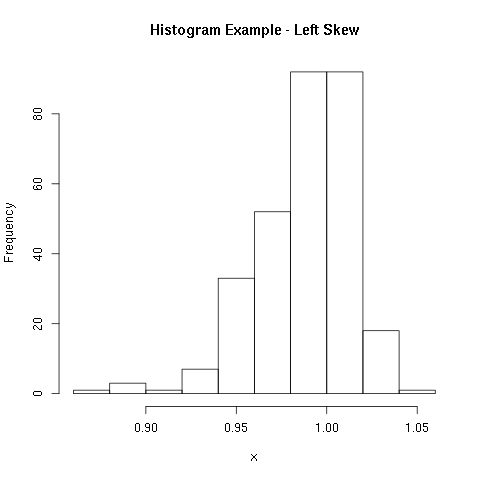
\includegraphics[width=7cm]{img/leftSkew}
  }

  \only<2>%
  {
    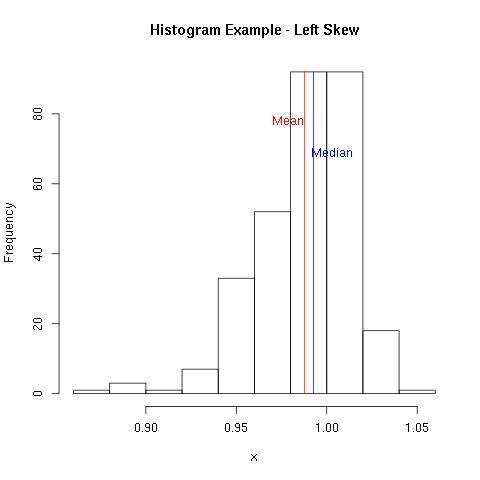
\includegraphics[width=7cm]{img/leftSkewAnnotated}
  }

  
\end{frame}


\begin{frame}{Skewed to the Right}

  \only<1>%
  {
    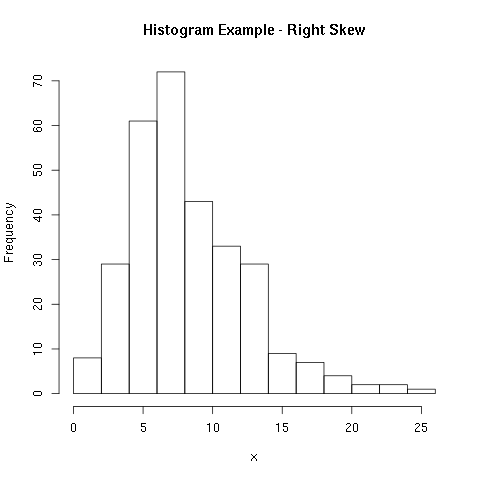
\includegraphics[width=7cm]{img/rightSkew}
  }

  \only<2>%
  {
    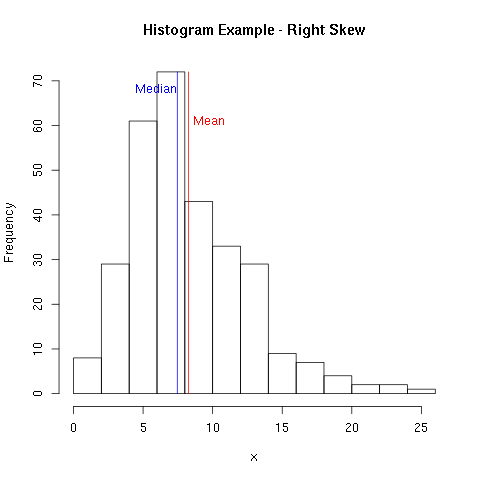
\includegraphics[width=7cm]{img/rightSkewAnnotated}
  }

  
\end{frame}


\begin{frame}{Symmetric}

  \only<1>%
  {
    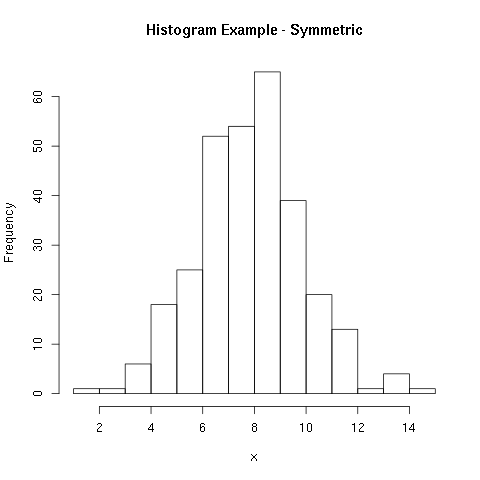
\includegraphics[width=7cm]{img/symmetric}
  }

  \only<2>%
  {
    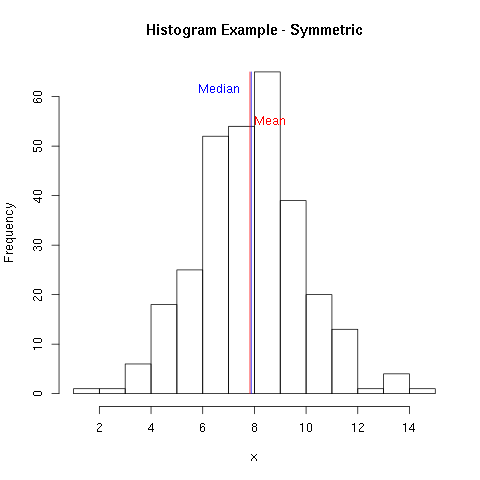
\includegraphics[width=7cm]{img/symmetricAnnotated}
  }

  
\end{frame}


\subsection{Spread of Data}

\begin{frame}{Center of what?}

  The sample mean and sample median give us an estimate of the
  ``center'' of the data. The question that next comes up is the
  center of what?

  The center of the data is just as important as the spread around the
  center.
  
\end{frame}

\begin{frame}{Example}

  You have daily sales from stores. You take ten samples from each store and
  want to estimate the mean sales. For which store do you place a
  greater trust in your estimate?

  \begin{columns}
    \column{.5\textwidth}
    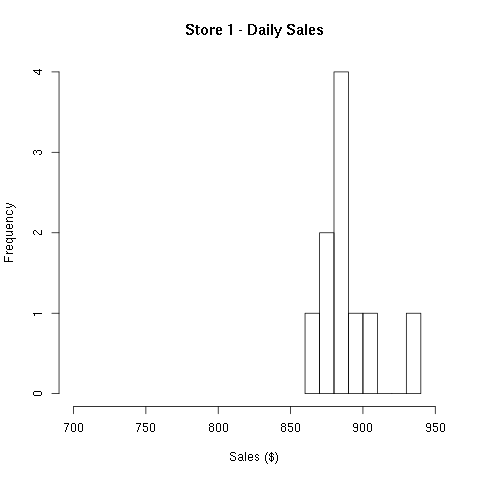
\includegraphics[width=4cm]{img/dailySalesStore1}

    \column{.5\textwidth}
    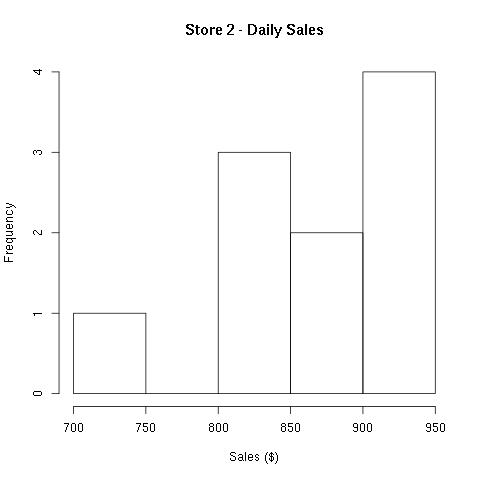
\includegraphics[width=4cm]{img/dailySalesStore2}
    
  \end{columns}
  
\end{frame}

\begin{frame}
  \frametitle{Spread of Data}

  Given data:
  \begin{eqnarray*}
    x_1, ~ x_2, ~ x_3, ~ \ldots ~,x_n.
  \end{eqnarray*}

  \begin{definition}
    The sample range is the biggest number minus the smallest number.
  \end{definition}


  \begin{definition}
    The sample variation of the data is 
    \begin{eqnarray*}
      s^2 & = & \frac{(x_1-\bar{x})^2+(x_2-\bar{x})^2+\cdots+(x_n-\bar{x})^2}{n-1}.
    \end{eqnarray*}
  \end{definition}

  \begin{definition}
    The sample standard deviation of the data is the square root of
    the sample variation.
  \end{definition}


\end{frame}

\begin{frame}{Example}

  Find the sample range and the sample standard deviation of the following data: \\
  \begin{tabular}{lll}
    3, & 5, & -2
  \end{tabular}

  
\end{frame}

\iftoggle{clicker}{%
  \begin{frame}
    \frametitle{Clicker Quiz}
    (Use channel 42)

    Find the sample standard deviation of the following data set:
    \vfill 

    \begin{tabular}{llll}
      3, & 3, & 2, & 4
    \end{tabular}

    \vfill

    \begin{tabular}{l@{\hspace{3em}}l@{\hspace{3em}}l@{\hspace{3em}}l}
      a: 0.5  & b: 0.667  & C: 0.707 & D: 0.816
    \end{tabular}

    \vfill

  

  \end{frame}
}







% LocalWords:  Clarkson pausesection hideallsubsections
